\section{Scénario de création d'un T.P. avec captures d'écrans}

Afin de commencer la préparation d’un TP dans la nouvelle architecture virtuelle, l’enseignant souhaitant proposer un TP à ses étudiants doit se connecter au serveur principal à l’aide de vsphère client.
Les comptes des enseignants disposeront de droits afin de pouvoir créer des template de VM permettant de générer les machines de TP. (Lors de la réalisation d’un TP, les étudiants se loggerons selon la même procédure, leurs comptes leur permettant uniquement d’administrer leurs machines personnelles et récupérer les machines virtuelles mises à disposition par les enseignants\\

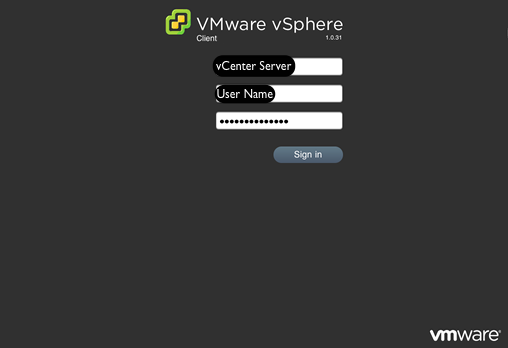
\includegraphics{Login.png}\\


Une fois connecté sur le vSphere Client, l’enseignant a accès à l’ensemble des puissants outils d’administrations fournis par VMware.
L’enseignant, afin de préparer son T.P., devra tout d’abord créer une machine virtuelle (ou en copier une existante, ce qui sera détaillé plus tard) correspondant aux besoins de son T.P. Il pourra par exemple créer une machine virtuelle dont l’objectif sera de permettre aux étudiants de réaliser des tâches d’administration réseau. Il lui suffit pour cela de cliquer sur File -> New -> Virtual Machine. L’assistant de création de machine virtuelle est alors lancé, et il suffit de suivre les indications pour créer la machine virtuelle.\\

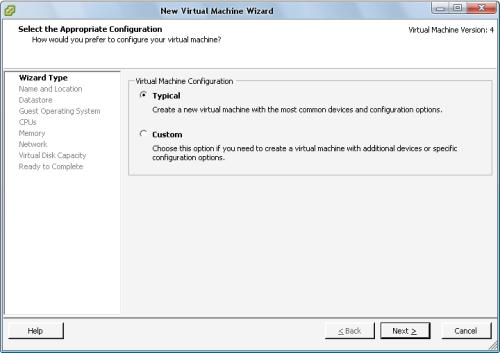
\includegraphics[scale=0.73]{newVM.png}\\

L’enseignant doit maintenant créer un template de machine virtuelle (clic droit sur la machine cible -> clone to Template). Ce template sera une machine virtuelle que les étudiants auront la possibilité de copier (cloner) afin de pouvoir travailler sur leur propre machine virtuelle. Afin que les étudiants puissent avoir accès à ce template, l’enseignant devra le place lors de se création dans un dossier auquel les étudiants ont des droits en lecture.\\

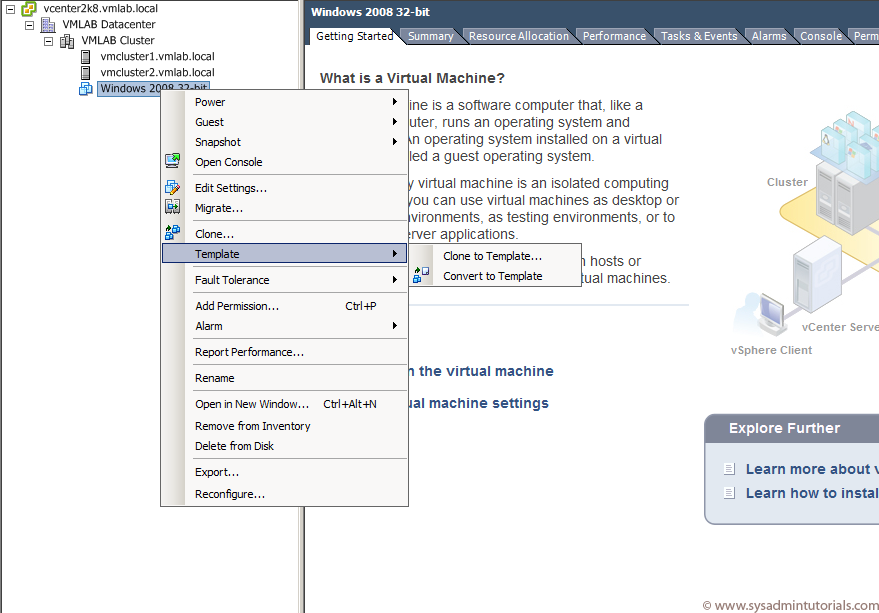
\includegraphics[scale=0.3]{template1.png}\\

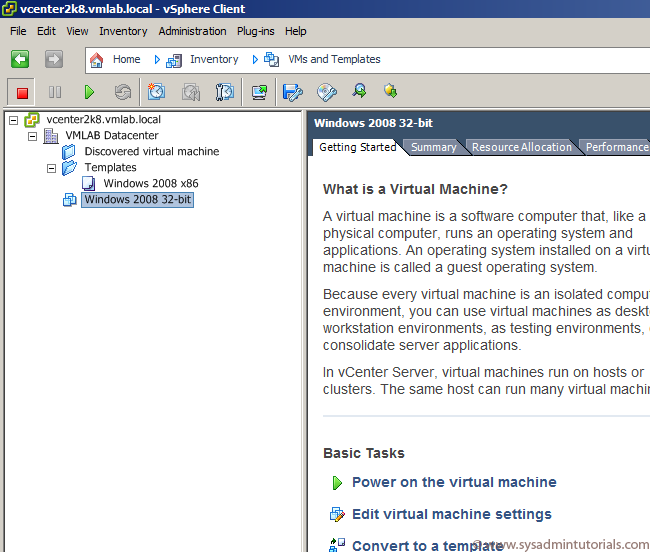
\includegraphics[scale=0.3]{template2.png}\\

Une fois la machine virtuelle créée par l’enseignant, lors de la première séance de TP, les étudiants devront, par groupe, cloner la VM afin d’en avoir chacun une à disposition. Le TP peut alors se dérouler comme un TP normal. L’enseignant pourra cependant facilement monitorer les travaux des étudiants en temps réel et les assister en ouvrant une deuxième console sur les VMs de travail.\\

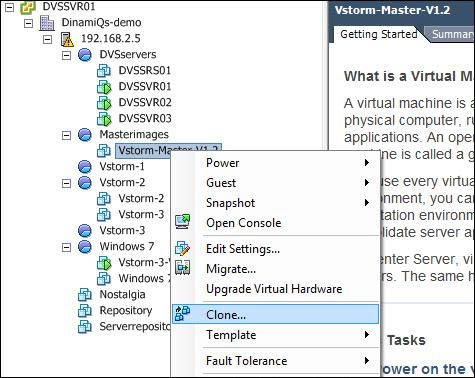
\includegraphics[scale=0.4]{clone.jpg}\\

Une fois le T.P. réalisé par l’étudiant, celui-ci devra prendre un snapshot de sa machine virtuelle. L’enseignant ayant accès à la machine virtuelle que l’étudiant a cloné, il lui suffira de restaurer l’état de la machine pour contrôler le travail de l’étudiant. Il aura évidemment la possibilité de vérifier l’heure à laquelle le snapshot a été pris, ou bien encore de retirer les droits d’écriture sur le dossier dans lequel l’étudiant doit créer sa V.M afin d’éviter toute fraude.\\

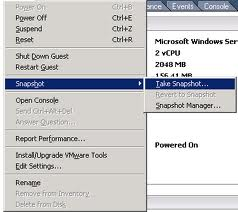
\includegraphics{snapshot.jpg}\\

Comme il est possible de la constater, l'utilisation de la plateforme pédagogique est extrèmement simple, et très intuitive. Les nombreuses fonctionnalités disponnibles (dont il est impossible de fournir une liste exhaustive dans ce document) devraient permettre aux utilisateurs de la plateforme pédagogique d'obtenir entière satisfaction de celle-ci.